\chapter{Motivation and a one-dimensional prelude} \label{sec:motivation}

In this section we will demonstrate how the Euclidean distance criterion in the TGO method disregards useful information about the (approximate) geometry of the objective function and we show how known information can be used effectively both in global optimisation and in mapping the local minima of objective functions as efficiently as possible. We also show how two important hyperparameters used by TGO, namely the number of sampling points $N$ and the choice of $k$ can be iteratively selected by intelligently exploiting information known from the topograph. This draws parallels to other works on iterative versions of TGO (I-TGO) \cite{Torn1996} trying to extract information from black-box objective functions. The informal, but intuitive ideas developed here will later be extended more rigorously to higher dimensional surfaces. Note that from Equation (\ref{eq:omega}) $\Omega$ is always a compact space, this fact is important in several proofs used in this Section. %, in \Cref{sec:shgo} we show that these ideas extend naturally to non-convex sets of $\Omega$ iff they contain any disconnected compact subspaces. %$ then if certain assumptions are made about the sampling sequence. 
\paragraph{Example 1}Consider the following objective function
\begin{equation} \label{eq:test1}
\underset{x}{\min} ~f(x) = \frac{\sin(x)}{x}, ~ x \in  \Omega = [1, 20]
\end{equation}
In this instance of the bounded optimisation problem there are 3 local minima which we will try to map in as few function evaluations as possible. 

Following the TGO procedure we start by generating low-discrepancy sampling points. The first $N = 10$ points in the 1-dimensional Sobol sequence is given by
$\mathcal{P} = \{
   p_{1}   =   1.0,  
   p_{2}   =   10.5,    
   p_{3}   =   15.25,   
   p_{4}   =   5.75,
   p_{5}   =   8.125,   
   p_{6}   =   17.625,    
   p_{7}   =   12.875, 
   p_{8}   =   3.375,   
   p_{9}   =   4.5625,   
   p_{10}   =   14.0625 \} \subset \Omega $.
After mapping the objective function at the set of sampling points    
\begin{equation}
f:
\begin{bmatrix}
   p_{1}   =   1.0 \\  
   p_{2}   =   10.5\\    
   p_{3}   =   15.25\\   
   p_{4}   =   5.75\\
   p_{5}   =   8.125\\   
   p_{6}   =   17.625\\    
   p_{7}   =   12.875\\ 
   p_{8}   =   3.375\\   
   p_{9}   =   4.5625\\   
   p_{10}   =   14.0625.
\end{bmatrix}
\rightarrow
\begin{bmatrix}
   f_{1}   =    0.84147\\
   f_{2}   =   -0.08378\\
   f_{3}   =    0.02899\\
   f_{4}   =   -0.08840\\
   f_{5}   =    0.11858\\
   f_{6}   =   -0.05337\\
   f_{7}   =    0.02359\\
   f_{8}   =   -0.06853\\
   f_{9}   =   -0.21672\\
   f_{10}   =   0.07091\\
\end{bmatrix}
\end{equation}
the corresponding topograph is constructed
\begin{equation}
\begin{bmatrix}[c|cccccccccc]
     p_{1}  &  -p_{8}  &  -p_{9}  &  -p_{4}  &  -p_{5}  &  -p_{2}  &  -p_{7}  &  -p_{10}   & -p_{3}  &  -p_{6} \\
     p_{2}  &  +p_{5}  &  +p_{7}  &  +p_{10}  &  +p_{3}  &  -p_{4}  &  -p_{9}  &  +p_{6}   & +p_{8}  &  +p_{1} \\
     p_{3}  &  +p_{10}  &  -p_{6}  &  -p_{7}  &  -p_{2}  &  +p_{5}  &  -p_{4}  &  -p_{9}   & -p_{8}  &  +p_{1} \\
     p_{4}  &  -p_{9}  &  +p_{5}  &  +p_{8}  &  +p_{1}  &  +p_{2}  &  +p_{7}  &  +p_{10}   & +p_{3}  &  +p_{6} \\
     p_{5}  &  -p_{2}  &  -p_{4}  &  -p_{9}  &  -p_{7}  &  -p_{8}  &  -p_{10}  &  +p_{1}   & -p_{3}  &  -p_{6} \\
     p_{6}  &  +p_{3}  &  +p_{10}  &  +p_{7}  &  -p_{2}  &  +p_{5}  &  -p_{4}  &  -p_{9}   & -p_{8}  &  +p_{1} \\
     p_{7}  &  +p_{10}  &  -p_{2}  &  +p_{3}  &  +p_{5}  &  -p_{6}  &  -p_{4}  &  -p_{9}   & -p_{8}  &  +p_{1} \\
     p_{8}  &  -p_{9}  &  +p_{1}  &  -p_{4}  &  +p_{5}  &  -p_{2}  &  +p_{7}  &  +p_{10}   & +p_{3}  &  +p_{6} \\
     p_{9}  &  +p_{4}  &  +p_{8}  &  +p_{1}  &  +p_{5}  &  +p_{2}  &  +p_{7}  &  +p_{10}   & +p_{3}  &  +p_{6} \\
    p_{10}  &  -p_{3}  &  -p_{7}  &  -p_{2}  &  -p_{6}  &  +p_{5}  &  -p_{4}  &  -p_{9}    &-p_{8}  &  +p_{1} \\
\end{bmatrix}
\end{equation}

The sampling points together with the objective function evaluations are plotted in \Cref{fig:pot1}. Using the empirical relation from \citet{Henderson2015} the optimal $k_c$ is calculated at $k_c = 8$. Using \Cref{def:tgo3} we find that the resulting $8$-$t$-matrix has only one minimiser; the global minimiser at $p_{9} = 4.5625$. For the local minimisation we use the SLSQP method as implemented in the function scipy.optimize.minimize \cite{scipy} to find the approximate global minimum at $x = 4.4934$. 

\begin{figure} [H] 
\centerline{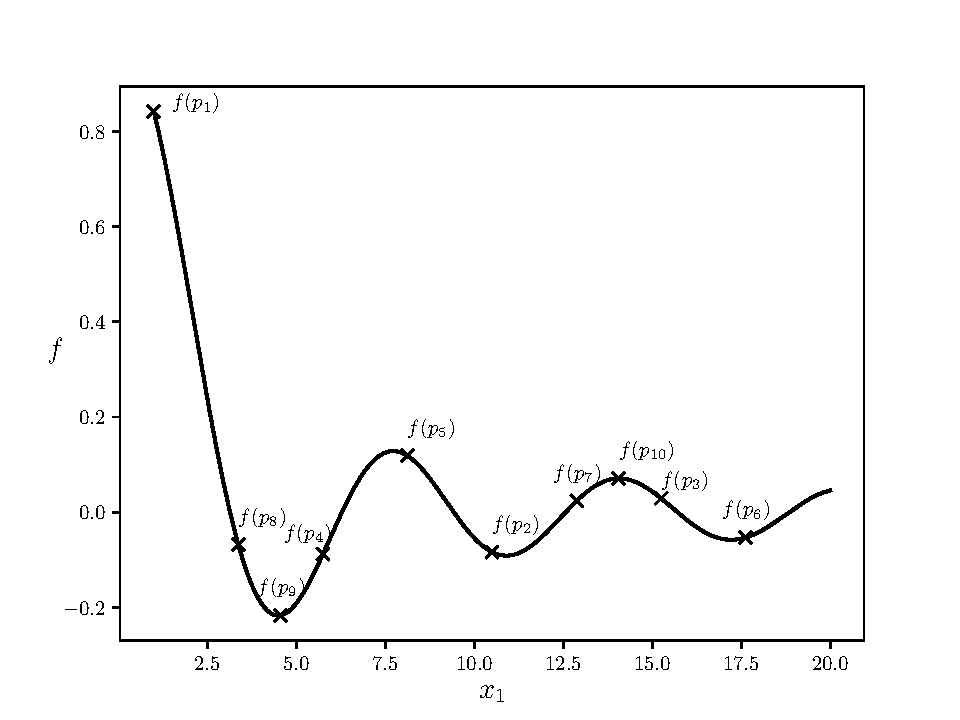
\includegraphics[scale=1.0]{./Fig1.pdf}}
{\caption{Test function give by Equation (\ref{eq:test1}) with 10 Sobol sequenced sampling points} \label{fig:pot1}}
\end{figure}

Observing \Cref{fig:pot1} it is immediately apparent that the set of 10 sampling points alone provides adequate information to deduce that there are at least 3 local minima. Observe that there are at least two other local minima since $ f(p_5) < f(p_2) < f(p_7)$. So at least one local minimum exists in the domain $(p_5, p_7) \subset \mathbb{R}$ since between $p_5$ and $p_2$ we must have, by the mean value theorem (MVT), $\frac{df}{dx} < 0$ for some domain $x \in [p_5, p_2] \subset \mathbb{R}$. Similarly for $x \in [p_2, p_7] \subset \mathbb{R}$ we have by MVT $\frac{df}{dx} > 0$. Since $f$ is a smooth, continuous function for $x \in (0, \infty)$ there must exist at least one stationary point $x  \in (p_5, p_7)  \subset \mathbb{R}$ where $\frac{df}{dx} = 0$. Furthermore we observe $f(p_6) < f(p_3)$ indicating another minimum in the domain $x  \in (p_3, 20] \subset \mathbb{R}$ since the minimum must be either on the boundary or in $x  \in (p_3, 20] \subset \mathbb{R}$ by the same argument as above. % !!TODO: offer a rigorous proof for these statements?!!  

The empirical relation by \citet{Henderson2015} was mainly developed for the purpose of finding the global minimum. Therefore if only $10$ sampling points are available, then in order to find more local minima using the TGO method, it is required to force a lower $k$ value. Alternatively, since $k_c$ is a function of $N$, simply sampling more points is sufficient to find all the local minima using Henderson's formula for this test problem. For example at $N=16$ all 3 local minima are produced by TGO with Henderson's formula. \Cref{fig:min} shows the number of minimisers found at different $k$ values for this example. The maximum minimiser set (other than using every sampling point as a starting point) can be trivially extracted by setting $k=1$ and calculating $|\mathcal{M}^1|$. However, in this Example it leads to more starting points than optimal since at least two minimisers will be in the same convex basin domain and therefore converge to same minimum in the local minimisation step. This results in superfluous function evaluations without extracting more useful information from the objective function. 

This idea drives the motivation behind the following definition.
\begin{definition} \label{def:optpool}
For a given set $\mathcal{P}$ of $N$ sampling points, $k_{opt}$ is any integer $1 \leq k \leq (N -1)$ that will produce the optimal minimiser set $\mathcal{M}^{k_{opt}}$ containing the maximum set of minimisers such that no two starting points extracted from $\mathcal{M}^{k_{opt}}$ will lead to the same minimum in the local optimisation step for some tolerance $\epsilon$. In other words every element contained in $\mathcal{M}^{k_{opt}}$ should lie in a unique locally convex sub-domain.
\end{definition}

Note that for a given $N$, $\mathcal{M}^{k_{opt}}$ might not produce all the true local minima of an objective function. What's important is that, given the information known from the sampling, the maximum number of local minima are found. In addition, no function evaluations are wasted in the local minimisation step which lead to the same minimum.

% !!TODO: THIS IS NOT WRITTEN IN TORN1992 FIND ANOTHER REFERENCE:  This flaw in the TGO algorithm is not unknown, \citet{Torn1992} noted the trade-off between using more local minimisers and the associated computational cost concluding that a larger $k$ value will lead to more function evaluations in the local search step without significant contributions.!!!

\begin{figure}
\centerline{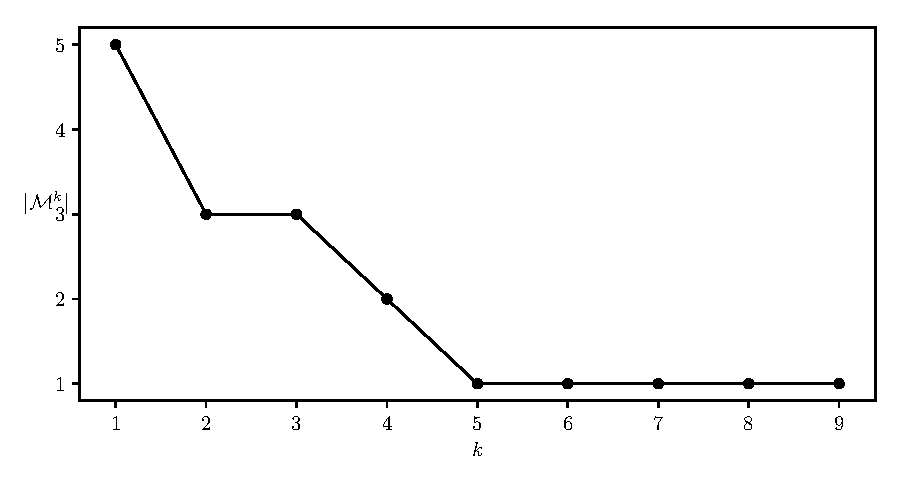
\includegraphics[scale=1.0]{./Fig2.pdf}}
{\caption{Number of minimisers $|\mathcal{M}^k|$ found using the TGO method for different $k$ values at $N = 10$}  \label{fig:min}}
\end{figure}

In Example 1 for $N = 10$ the optimal $k$ values are $k_{opt}=\{2, 3\}$ which will produce 3 minimisers $|\mathcal{M}^2| = |\mathcal{M}^3| = 3$. We will now show that these lower $k$ values carry unexploited information on the best approximate geometry for the objective function. For example in \Cref{fig:mink} we plot the $|\mathcal{M}^k|$ values corresponding to the set $k = \{1, 2, 3, 4, 5, 6, 7, 8, 9, 10\}$ for every sampling point range $N \in [2, 50]$.

\begin{figure} 
\centerline{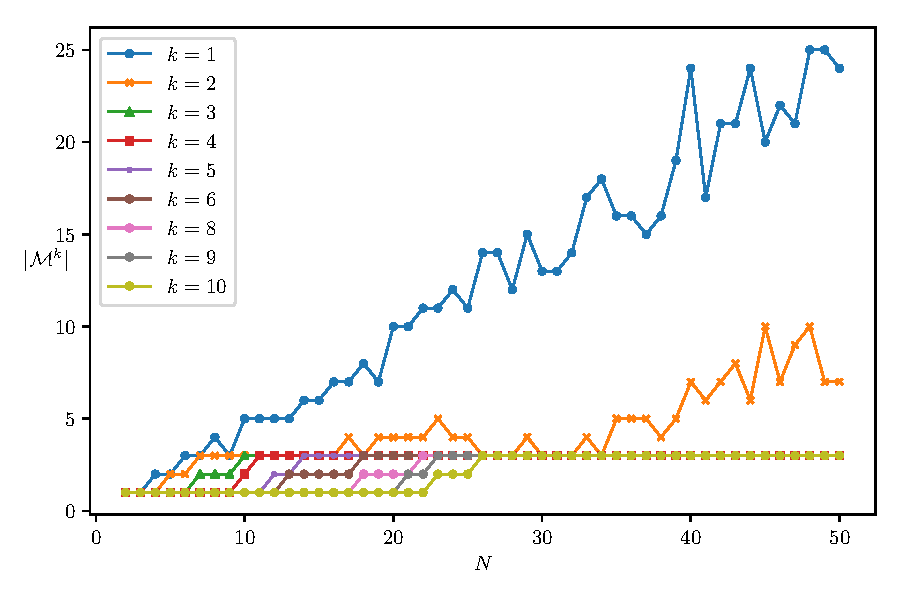
\includegraphics[scale=1.0]{./Fig3.pdf}}
{\caption{Number of minimisers $|\mathcal{M}^k|$ found using the TGO method for the given $k$ values at various sampling points $N$} \label{fig:mink}}
\end{figure}

From \Cref{fig:mink} we notice the special property of $k = 3$ for one dimensional objective functions sampled with the Sobol sequence. 

Firstly, for a lower number of sampling points $N$ it provides a higher number of starting minimisers than $k > 3$. Note that by inspection of Definition \ref{def:tgo3} it can be determined that any $k > 3$ value will always produce an equal or lower number of minimisers than $k = 3$ (this is also true for any $k > i$). When adding columns to a positive row there are only two possibilities: the next sampling point in the row can either have a positive or a negative sign. All other elements in the row have a positive sign by definition (see Definition \ref{def:tgo3}). If the next sampling point in the row has a positive sign then the row will just remain a positive row and the number of minimisers remain the same. If the point is a negative reference point then the row will no longer be a positive row and thus the point is no longer a minimiser, lowering the total.

Secondly it can be observed that $k = 3$ never calculates a number of starting minimisers higher than optimal unlike $k < 3$. Therefore by using $k = 3$ in Example 1 TGO will always find as many minimisers in as few sampling\footnote{not necessarily total function evaluations since starting points closer to the local minima may provide better performance for a given local minimisation routines} function evaluations as possible and furthermore all local minima will be found when $N \ge 10$. It should be noted that the total number of function evaluations depends on the particular local minimisation algorithm used. However, it is apparent that each minimiser starting point is in a unique locally convex domain. It is tempting for an optimisation practitioner to use the size of the set of minimisers $|\mathcal{M}^3|$ as a stopping criterion for iterative sampling $N$ of one dimensional objective functions. The practical usefulness of this idea can be demonstrated with the following example:

\paragraph{Example 2} The following instance of the optimisation problem has 13 local minima in the given domain
\begin{equation} \label{eq:test2}
\underset{x}{\min} ~f(x) = -x \sin(x), ~ x  \in  \Omega = [1, 80]
\end{equation}

From \Cref{fig:mink2} we can deduce that the minimum number of sampling points required for $k = 3$ to find all local minima using the Sobol sequence is $N = 40$, this sampling is shown in \Cref{fig:pot2}.  If  $N < 40$ then there aren't enough sampling points to deduce that there are at least 13 locally convex domains from using the same arguments as in Example 1. Note for example that if we used a sequence that skipped $p_1$ then $N =39$ would be adequate since $l = 1 < p_{32} < p_{33}$. Using our Python implementation of TGO \cite{TGOpy} with $N = 40$ all 13 local minima of the objective function were found in a total of 285 function evaluations. 

An example of a stopping criterion would be to stop sampling if $|\mathcal{M}^3|$ is unchanged after, say, 10 sampling point evaluations. The rate at which the number of elements in $|\mathcal{M}^3|$ grows with increasing $N$ also provides a heuristic for characterising the multimodality and the geometry of the objective function. Objective functions that have a large number of local minima in a small domain (and relatively fewer minima in other larger domains) will have a much smaller growth in $|\mathcal{M}^3|$ for a given low-discrepancy sampling. This idea of continuously classifying and extracting approximate function characteristic information from the sampling points will be formalised and extended to higher dimensions in \Cref{sec:shgo}.


\begin{figure}  \label{fig:mink2}
\centerline{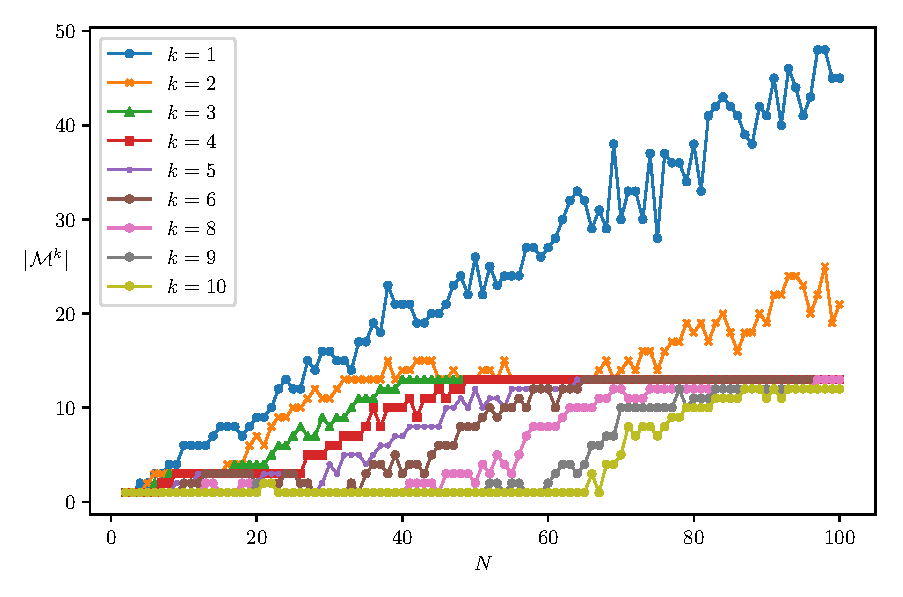
\includegraphics[scale=1.0]{./Fig4.pdf}}
{\caption{Number of minimisers $|\mathcal{M}^k|$ found using the TGO method for the given $k$ values at various sampling points $N$}  \label{fig:mink2}}
\end{figure}

\begin{figure} 
\centerline{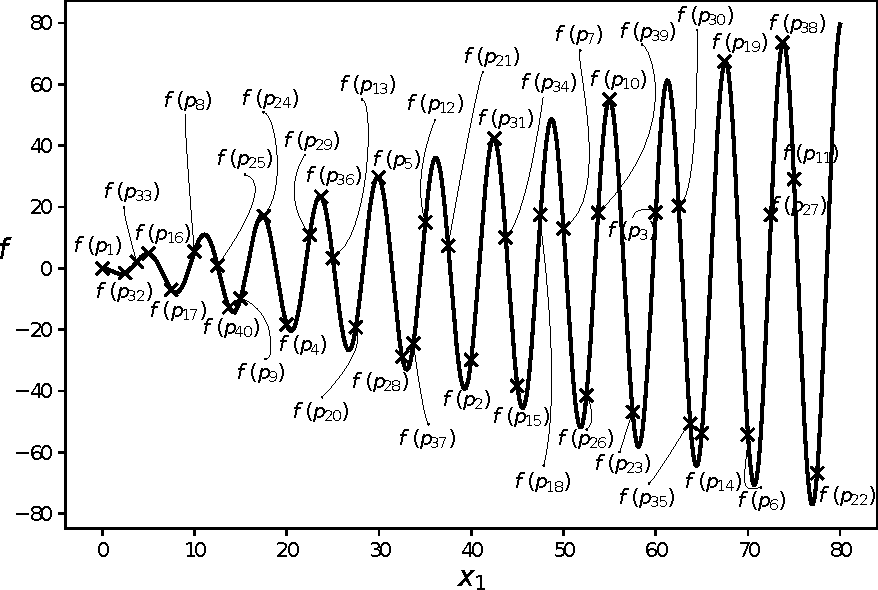
\includegraphics[scale=1.0]{./Fig5.pdf}}
{\caption{Plot of the objective function in Example 2 for $N = 40$ sampling points} \label{fig:pot2}}
\end{figure}

There is a simple reason why the $3$-$t$-matrix has this quality in the first dimension for the optimisation problem given in Equation (\ref{eq:test1}). However, it is not guaranteed that this property holds for any sampling point distribution. In fact it holds true only under the following conditions:
\begin{enumerate}
\item Consider all points in the ordered sampling set from the smallest to greatest $x$ value $\mathcal{P} = \{p_i~|~p_{0}~<~p_{1}~<~p_{2}~\dots~<~p_N-1,~p_{i}~\in~(x_l,~x_u)\}$, excluding the supremum and infimum.
\item For any given point $p_i$ the Euclidean distance between $p_i$ and 2 of its nearest sampling points $p_{i-1} < p_i < p_{i+1}$ should be less than the relative difference between $p_i$ and a fourth point in the sampling sequence $|p_i - p_j|$ where $j \neq {i, i-1, i+1}$.
\end{enumerate}
 
In fact it is easy to prove both that for a locally, strictly convex domain of $f$ the $3-$topograph construction can produce a larger minimiser pool $\mathcal{M}^3$ than optimal. It can also be shown that a construction must exist where the optimal number of minimisers will \it{always} \normalfont be extracted regardless of the sampling distribution. Furthermore it can be shown that at most 3 sampling points within a locally convex domain $x \in [x_l, x_u]$ is required to produce enough information so that only one minimiser in the domain is produced.

\begin{theorem} \label{1d}
There exists a $1$-dimensional sampling sequence such that $k = 3$ will produce a minimiser pool larger than optimal as defined by Definition \ref{def:optpool}.
\end{theorem}

\begin{proof}
Consider a subdomain $x \in [x_l, x_u] \subset \mathbb{R}$ for which $f$ is strictly convex. We define the set of $N$ sampling points $\mathcal{P}$ ordered in such a way that $$\mathcal{P} = \{p_i~|~p_{0}~<~p_{1}~<~p_{2}<~\dots~<~p_{N-1},~p_{i}~\in~(x_l,~x_u)\}$$

Let $\mathcal{F} = \{f_{0},~f_{1},~f_{2},\dots,~f_{N-1}\}$ be set of one-to-one function values corresponding to the points mapped by $f:\mathcal{P} \rightarrow \mathcal{F}$. 

Suppose we have $f_1 < f_0$ and $f_1 < f_2 < f_3, \dots f_{N-1}$.  %, by construction we have  $|p_i - p_j|$
By construction we have  $|p_1 - p_2| < |p_1 - p_3| < |p_1 - p_4| < |p_1 - p_5|$ then by the Definitions \ref{def:tgo1}, \ref{def:tgo2} and \ref{def:tgo3} $p_2$ is a minimiser of the $3-t-$topograph. Suppose we have a sampling distribution such that $|p_2 - p_3| < |p_1 - p_2|, |p_2 - p_4| < |p_1 - p_2|$ and $|p_2 - p_5| < |p_1 - p_2|$ then by the Definitions \ref{def:tgo1}, \ref{def:tgo2} and \ref{def:tgo3} $p_3$ is also a minimiser of the $3-t-$topograph. Therefore more than two minimisers are produced in the same locally convex sub-domain of $[x_l, x_u]$. We have shown that $\mathcal{M}^3$ can produce a minimiser pool larger than optimal which concludes the proof.

\begin{lemma} \label{1dax}
A construction exists that will always produce a minimiser pool larger than optimal as defined by Definition \ref{def:optpool} for any given $1$-dimensional sampling sequence.
\end{lemma}

Now suppose that instead of using only the Euclidean distance metric we also invoke knowledge of the nearest point in all cartesian directions. We use the criterion that a minimiser point $p_i$ is a minimiser iff \normalfont with the ordering constructed in $\mathcal{P}$ and $\mathcal{F}$ we have $f_i < f_{i - 1}$ and $f_i < f_{i + 1}$. With this definition if the point $p_i$ is a minimiser then no other point meets the criterion since by construction of the sampling in the locally convex domain $f_{0} > f_{1} > \dots > f_{i - 1} > f_i$ and $f_{i + 1} < f_{i + 2} < f_{i + 3} < \dots < f_{N-1}$. This proves Lemma \ref{1dax}. 

Finally note that only information from the 3 points in the locally convex sub-domain of $[x_l, x_u]$ and their corresponding function values $f_{i - 1}$, $f_{i}$ and $f_{i + 1}$ are needed to produce a minimiser using this criterion.
\end{proof}

There is an important consequence here for low discrepancy sequences in higher dimensions and for less well behaved objective functions. In both these cases. the topographs connected with the Euclidean distance metrics will discard available information about the local geometry of the objective function surface. This produces larger than optimal minimiser pools leading to very high numbers of function evaluations needed to solve the problem.


%!! TODO: Add visual aide, motivate that this kind of shitty distribution will happen in higher dimensions even for good sequences like Sobol. \\


%Clearly in using the Euclidian distance matrix the information known by contruction (the relative position of the sampling points on the $x$-axis) is lost

%Since the $x$ variable can only vary in one positive or negative direction, however, in higher dimensions...



In the following section we will develop a more efficient algorithm that will make use of this information. SHGO will always produce equivalent results to this algorithm in the one dimensional case.
